\section{Software Engineering Method}
\label{sec:software_engineering_method}
This section will shortly describe the software engineering method used during this project, how it was chosen and how we intend to implement it into our project.

\subsection{Choosing a Development Method}
There exist many different development methods, such as Scrum, \ac{xp}, \ac{up}, and the classic waterfall method.
This project rely heavily on initial analysis before starting to design and implement, since the problem was not clearly defined from the beginning.
Using \ac{xp} to instantly write code would therefore not be suitable for this project, and for that reason, it was quickly discarded.
Scrum is suitable to implement in projects where requirements to the final project often change.
It includes cycles, called sprints, that include analysis, design, implementation and testing.
We did not feel, that Scrum was suitable for our project, since the requirements, when determined, are fairly static.
The static nature of the requirements might make it possible to implement the classical waterfall method, but given our prior knowledge from lectures, the waterfall method is generally not very usable and potentially limiting by having to declare on part of the process finished before starting the next.
Therefore, we decided to use \ac{up} as the development method.
\ac{up} divides the software development processes into the following four phases: 

\begin{itemize}
\item[Inception] The project's boundaries and scope should be defined, as well as risk identification and preliminary project schedule.
\item[Elaboration] The team is expected to create the majority of the system requirements and establish the system architecture.
\item[Construction] This should be the largest phase in the project, since this is where the system is implemented.
\item[Transition] The project is deployed and feedback is incorporated into future releases.
\end{itemize}

Each phase is divided into iterations and will contain most of the activities associated with software development (analysis, design, implementation and testing), but to varying degrees. As can be seen in\autoref{fig:up}, the main focus will gradually shift from one activity to the next in the process.\todo{Barbara: Source of picture please}

\begin{figure}[ht]
  \centering
    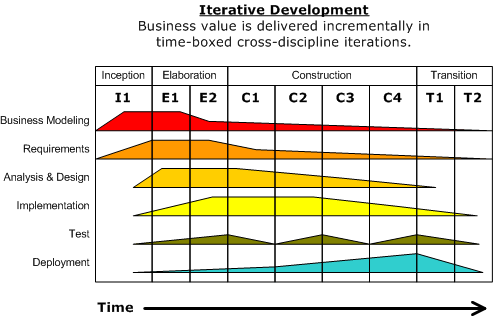
\includegraphics[width=\textwidth]{img/Development-iterative.png}
  \caption{Phases and activities in UP}
  \label{fig:up}
\end{figure}

%Given that this project is estimated to require a long time spent on analysis before actual development can take place, an iterative method with short cycles spent on all activities, such as SCRUM, would not be suitable for this project. XP as a possible development method can also be discarded for the same reason.\newline
%Instead the group will begin by focusing on the analysis, definition and scope of the problem to be solved. It will then move on to design of the solution along with prototype implementation and testing of these. Finally the product will be tested and findings during the testing will be implemented. 

The fact that \ac{up} is divided into phases that each have iterations fits well with the group's wish to focus mostly on one development activity at a time, without using the dated classical waterfall structure of the project.
\ac{up} also initially focuses on requirements and analysis, which is suitable for this project.\newline

Now we will describe how we intend to implement \ac{up} into our project.

\subsection{Implementing UP}


\subsubsection{Inception}


\subsubsection{Elaboration}


\subsubsection{Construction}


\subsubsection{Transition}

